\section{MILP tolerance} \label{app:MILP}
In this Appendix, the impact of the modeling of the electrolysers with SOS2 variables is evaluated. The objective is to check that the operating points of the electrolysers on the obtained results do not deviate from the operating curve of \autoref{fig:ely_operating_range}. The gap between operating point given by the EMS and operating curve is calculated with Equation (\ref{eq:L2}). \autoref{fig:ely_gap} provides a visual representation of the gap, demonstrating that only a few operating points are significantly outside the allowed range. 
\begin{equation*}
     \text{Gap}_t = \textbf{L}_\textbf{t}^{\textbf{(k,elec)}} \cdot \alpha_i^{(k)} - \textbf{l}_\textbf{t}^{\textbf{(k,state)}} \cdot \beta_i^{(k)} - \textbf{L}_\textbf{t}^{\textbf{(k,H$_2$)}}
\end{equation*}
Despite minor deviations, the solutions remain close to the operating curve, attesting to the effectiveness and reliability of the MILP-based optimization approaches in achieving near-optimal EMS operation while adhering to constraints.\\

It is worth mentioning here that for all the results obtained, the solver used is CPLEX 22.1.0 and the relative gap between the solution returned and the optimal solution is notably small, with a value of 0.01 for both the \textit{Myopic} and \textit{Price Signal} approaches and an even smaller value of 0.001 for the \textit{Multiple RP-CF approach}. The reduced tolerance for RP-CF can be attributed to the consideration of long-term cost, requiring higher precision in the optimization process.

\begin{figure}
    \centering
    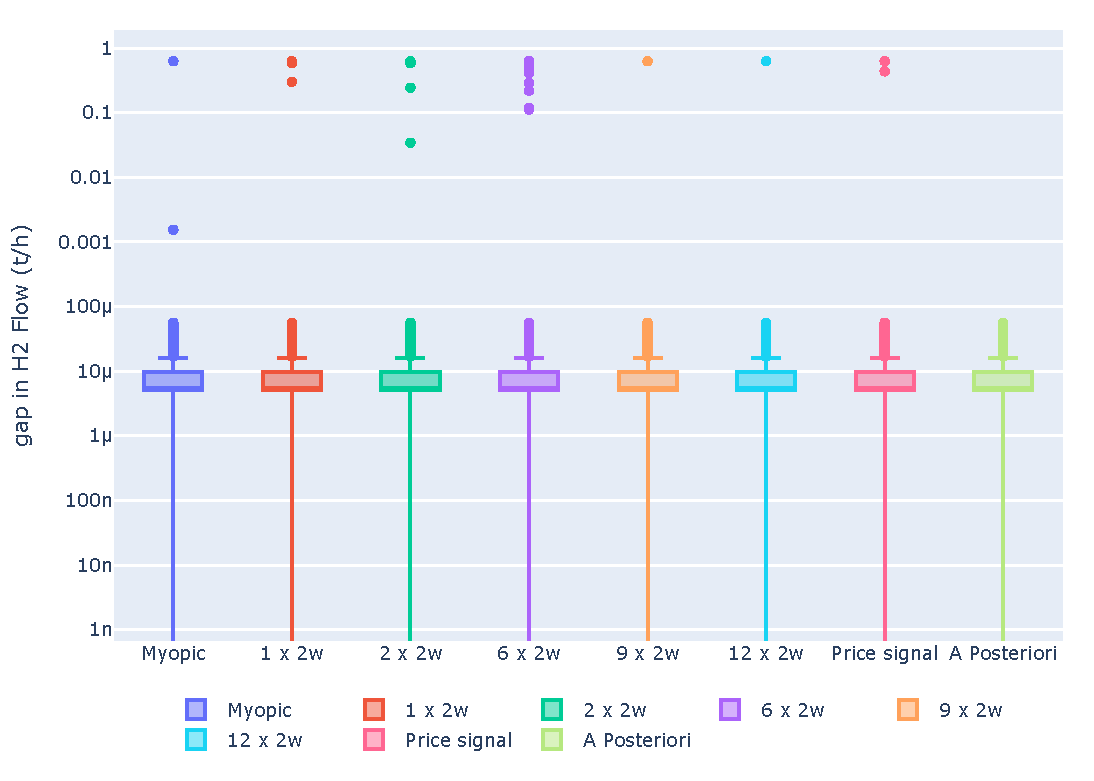
\includegraphics[width=10cm]{02_Appendix/MILP_tolerance_boxplot.pdf}\\
    \caption{Absolute gap between operation range of electrolyser and operating point of the EMS}
    \label{fig:ely_gap}
\end{figure} 